\documentclass[10pt, letterpaper]{article}
%Graphic and Diagram Setup
\usepackage[margin=1in]{geometry}
\usepackage{graphicx}
\usepackage{tikz}
\usepackage[all]{xy}

\usepackage{pdflscape}
\usepackage{rotating}

%Inserting Graphics
%An example of the use of this command is
% \begin{minipage}{4in}
%   \Fig{filename}
% \end{minipage}
\newcommand{\Fig}[1]{\includegraphics[width=0.5\textwidth]{#1}}

%Math Symbol Setup
\usepackage{ulem}
\usepackage{amsmath}
\usepackage{amsthm}
\usepackage{amssymb}

%Math Fonts
\usepackage{amsfonts}
\usepackage{mathrsfs}

%Absolute Value and Norm Notation
\newcommand{\abs}[1]{\left \lvert #1 \right \rvert}
\newcommand{\norm}[1]{\left \lVert #1 \right \rVert}

%Kernel of a map
\renewcommand{\ker}{\operatorname{Ker}}

%Lie Algebra of a Lie Group
\newcommand{\lie}[1]{\operatorname{Lie}(#1)}

%Fields and Blackboard Letters
\newcommand{\field}[1]{\mathbb{#1}}
\newcommand{\A}{\mathbb{A}}
\renewcommand{\P}{\mathbb{P}}
\newcommand{\N}{\mathbb{N}}
\newcommand{\Z}{\mathbb{Z}}

%Theorems and Definitions
\newtheorem{thm}{Theorem}
\newtheorem{lemma}{Lemma}
\newtheorem{cor}{Corollary}
\newtheorem{prop}{Proposition}

\theoremstyle{remark}
\newtheorem{rem}{Remark}

\theoremstyle{definition}
\newtheorem{defn}{Definition}
\newtheorem{ex}{Example}

%Fancy Header Setup
\usepackage{fancyhdr}
\fancyhf{}
\pagestyle{fancy}
\lhead{}
\chead{\bfseries Graph Theory, Minimal Spanning Trees \& Algorithms}
\rhead{}
\lfoot{Graph Theory \& Algorithms}
\cfoot{Eric Ebert}
\rfoot{\thepage}
\renewcommand{\headrulewidth}{0.5pt}
\renewcommand{\footrulewidth}{0.1pt}

%Double Space
\usepackage{setspace}
\linespread{1.6}

%Document Content
\begin{document}

\section{General Facts about Trees}

\begin{lemma}
	If $T$ is a tree then $T$ has a leaf.
\end{lemma}

\begin{proof}
	A leaf with vertex $v$ has degree 1. Suppose that $T$ does not have a leaf. Then the $\operatorname{deg}(v) \geq 2$
	for every $v \in V$. Hence, we can enter and leave every vertex on a different edge. Now construct a walk starting
	at $v_1$. We can then exit $v_1$ to another vertex $v_{i_1}$. We can keep doing this to get a sequence
	\[
		w = v_1 v_{i_1} v_{i_2} \cdots v_{i_k}
	\]
	When we get to $v_{i_k}$ we can leave and go to one of its neighbors. Because $V$ is finite, the pigeonhole
	principle tells us that eventually we've gone through some vertex twice. Hence, there exists a cycle in $T$. This
	is a contradiction as a tree is acyclic.
\end{proof}

\begin{lemma}
	Every tree has $\#V-1$ edges.
\end{lemma}

\begin{proof}
	We proceed by induction.

	\begin{itemize}
		\item [] \textbf{Base Case:} Let $T$ be a tree with two vertices. There is one edge incident to those two
		vertices as $T$ contains no cycles; $\# V-1 = 2-1 = 1$.
		\item [] \textbf{Inductive Hypothesis: (IH)} Suppose a tree $T$ with $k$ vertices has $k-1$ edges.
		\item [] \textbf{wts:} A tree with $k+1$ vertices has $k$ edges.
		Let $T$ be a tree with $k+1$ vertices and $v$ be a leaf. Remove the unique edge incident to $v$. This graph
		has $k$ vertices. By the IH, we know that it has $k-1$ edges. Now add $v$ and its edge to conclude that $T$ has
		$k$ edges.
	\end{itemize}
\end{proof}

\begin{prop}
	Let $G$ be a graph. The following are all equivalent:
	\begin{enumerate}
		\item $G$ is a tree.
		\item $G$ is connected and has $\# V-1$ edges.
		\item $G$ has no cycles and has $\# V-1$ edges.
		\item There is a unique path between any two vertices.
	\end{enumerate}
\end{prop}

\begin{proof}
	$(1) \Rightarrow (2)$ We've proven that a tree has $p-1$ edges and $G$ is connected by definition of a tree. \\
	$(2) \Rightarrow (3)$ $G$ has $\#V-1$ edges by assumption. Suppose that $G$ has a cycle $C$. Then there are at least
	three edges incident to two vertices. Then there are $\#V - 4$ edges for $\#V-3$ vertices.By the pigeonhole principle
	some vertex is isolated which implies that the graph $G$ is disconnected. We've arrived at a contradiction from the
	assumption that $G$ is connected.\\
	$(3) \Rightarrow (4)$ If there are two different paths between vertices $v_i$ and $v_j$, then there are vertices $v_k$
	and $v_{k'}$ that belong to one path but not both. For two paths
	\begin{align*}
		w &= v_i v_{s_1}v_{s_2} \cdots v_k \cdots v_{s_k}v_{s_{k+1}}v_j \\
		p &= v_i v_{t_1}v_{t_{2}} \cdots v_{k'} \cdots v_{t_k}v_{t_{k+1}}v_j \\
	\end{align*}
	If the $v_{s_k}$ and $v_{t_j}$ are all different then $w$ and $p$ form a cycle. Otherwise, there is a cycle
	containing the vertices $v_k$ and $v_{k'}$. This cycle can be constructed by deleting the vertices that are
	repeated in $p$ and $w$. This is a contradiction to our assumption that $G$ contains no cycles.
	$(4) \Rightarrow (1)$ If there existed a cycle there would be vertices $v_i$ and $v_j$ that had two different paths
	between them. Hence, the graph is acyclic. That every pair of vertices has a unique path connecting them implies
	that the graph is connected.
\end{proof}

\section{Spanning Trees}

\begin{defn}
	For a graph $G = \langle V,E \rangle$, a spanning tree $T$ for $G$ is an acyclic subgraph of $G$ that is connected.
\end{defn}

A spanning tree for a graph $G$ can be seen as:
\begin{enumerate}
	\item A tree $T$ which contains all of the vertices in $V$ and each edge of $T$ is also an edge of $G$.
	\item A maximal set of edges from $E$ that contains no cycle.
	\item A minimal set of edges that connect all vertices.
\end{enumerate}

Fix a spanning tree $T$. The \textit{cotree}, which we will denote by $\bar{T}$, is the set of edges in $E$ which do
are not edges of $T$. Adding an edge from $\bar{T}$ to $T$ will create a cycle $C_e$, where $e$ is an edge in $\bar{T}$.
The cycle $C_e$ is a \textit{fundamental cycle} of $G$. Because the edges in $\bar{T}$ are in one-to-one correspondence
with the fundamental cycles, these edges can be seen as a basis for the \textit{cycle space}.

On the other hand, if we delete an edge from $T$ the tree $T$ becomes disconnected. That is, every edge of a tree is
a cut edge. The vertices are now partitioned into two sets corresponding to the connected components. A
\textit{fundamental cut} is the set of edges that need to be deleted from $G$ to accomplish the same partition. Agalogous
to what we did above, the fundamental cuts and the branches of the tree are in one-to-one correspondence. The fundamental
cuts form a basis for the \textit{bond space}.

\section{Minimal Spanning Trees}

\begin{defn}[Minimal Spanning Trees]
Let $G$ be a connected edge weighted graph. A minimum spanning tree (MST) of $G$ is a subset of the edges traversing all vertices, with the minimal possible total edge weight, and is acyclic.
\end{defn}

We now consider a weighted version of our graph:

\begin{figure}[h]
	\centering
	
	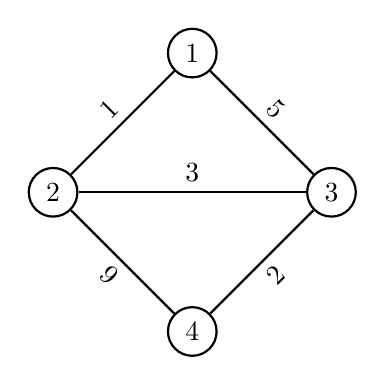
\begin{tikzpicture}[node distance={25mm}, thick, main/.style={draw,circle}]
		\node[main] (1) {$1$};
		\node[main] (2) [below left of = 1] {$2$};
		\node[main] (3) [below right of = 1] {3};
		\node[main] (4) [below right of = 2] {4};

		\draw (1) -- node[midway, above, sloped] {1} (2);
		\draw (1) -- node[midway, above, sloped] {5} (3);
		\draw (2) -- node[midway, above] {3} (3);
		\draw (2) -- node[midway, below, sloped] {9} (4);
		\draw (3) -- node[midway, below, sloped] {2} (4);
	\end{tikzpicture}

	\caption{Weighted Graph}
\end{figure} 

\begin{prop}[Cut Property]
For any cut $K$ of $G$, the edge in $K$ with the least (strictly smaller than all others) weight must belong to all MST.
\end{prop}

\begin{prop}[Cycle Property]
Given a cycle $C$ in $G$, the edge in $C$ with the largest weight cannot belong to an MST.
\end{prop}

\begin{prop}[Minimum Weight Edge Property]
If the edge with the least weight is unique, then this edge belongs to every MST.
\end{prop}


\end{document}
